\section{Signed og unsigned tal}
%  |
Når en unsigned værdi konverteres til en signed værdi, er most significant bit, den bit der bestemmer om tallet er negativt eller positivt.
Denne bit har værdien $-8$, når den er signed, og derved subtraheres der for alle yderligere bits.
\begin{table}[h]
    \centering
    \begin{tabular}{c|c|c|c}
        Bits&Unsigned&Signed&Hex\\\hline
        0000&0&0&0x0\\
        0001&1&1&0x1\\
        0010&2&2&0x2\\
        0011&3&2&0x3\\
        0100&4&4&0x4\\
        0101&5&5&0x5\\
        0110&6&6&0x6\\
        0111&7&7&0x7\\
        1000&8&-8&0x8\\
        1001&9&-7&0x9\\
        1010&10&-6&0xA\\
        1011&11&-5&0xB\\
        1100&12&-4&0xC\\
        1101&13&-3&0xD\\
        1110&14&-2&0xE\\
        1111&15&-1&0xF\\
    \end{tabular}
    \caption{Tabel over signed og unsigned værdier}
\end{table}
\begin{figure}[h!]
    \centering
    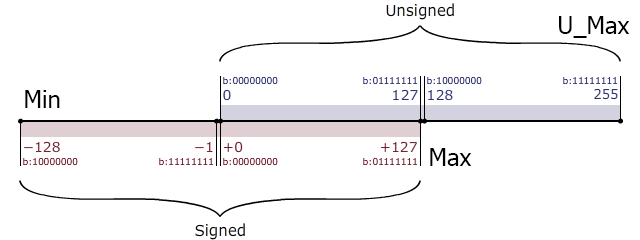
\includegraphics[width=\textwidth]{figures/signed.png}
    \caption{Signed og Unsigned komparativt}
    \label{fig:signed}
\end{figure}
